
\chapter{Resultados}
\label{ch:resultados}

Este capítulo presenta los resultados de la aplicación de
la metodología descrita en el Capítulo~\ref{ch:metodologia}
al universo de cooperativas de ahorro y crédito chilenas.
Los resultados se organizan en dos segmentos, en línea con
la distinción institucional vigente desde 2019: las CAC
no supervisadas por la CMF, cuya información financiera
proviene de balances y estados de resultados individuales
del portal DAES (segmento DAES); y las 7~CAC supervisadas
por la CMF, cuya información proviene de los estados
financieros anuales publicados por la CMF y de la
plataforma BEST (segmento CMF). % DESPUÉS:
Ambos segmentos se presentan primero por separado (secciones~\ref{sec:resultados-daes}
y~\ref{sec:resultados-cmf}), dado que corresponden a distintos períodos de
referencia y distintos regímenes de supervisión. La
sección~\ref{sec:agregado-total} presenta además un agregado conjunto, que
debe interpretarse como una aproximación de orden de magnitud --y no como
una suma metodológicamente estricta y exacta-- dadas las diferencias de
cobertura y período entre segmentos, documentadas en detalle en la
sección~\ref{sec:limitaciones}.
Los resultados se visualizan en el Dashboard Cuenta
Satélite CAC, desarrollado como parte de
este estudio, que permite explorar interactivamente las
series por entidad y por año para ambos segmentos. Disponible para descarga en \url{https://github.com/Iureta1/Dashboard_HuellaSocial}

% ============================================================
\section{Segmento DAES: CAC no supervisadas}
\label{sec:resultados-daes}
% ============================================================

\subsection{Cobertura del panel}
\label{subsec:cobertura-daes}
El panel del segmento DAES cubre el período 2014–2024 e incluye un total de 35~CAC
distintas, con una cobertura anual que oscila entre 2 y 22~entidades según la
disponibilidad de memorias en el portal DAES para cada ejercicio
(véase el Cuadro~\ref{tab:cobertura_daes}). Las variaciones interanuales reflejan
exclusivamente efectos de composición por disponibilidad de memorias, y no
necesariamente cambios en el universo activo del sector. La reducción a
11~entidades en 2024 obedece a que varias memorias de ese ejercicio no estaban
aún publicadas al momento del levantamiento. En ningún año el panel cubre la
totalidad del universo DAES, por lo que los agregados sectoriales constituyen
cotas inferiores del aporte real del segmento.

\begin{table}[H]
\centering
\caption{Cobertura anual del panel DAES}
\label{tab:cobertura_daes}
\small
\renewcommand{\arraystretch}{1.3}
\begin{tabularx}{\textwidth}{@{} c c X @{}}
\toprule
\textbf{Año} & \textbf{N} & \textbf{Nota de composición} \\
\midrule
2014 &  2 & Panel inicial; 2 CAC con al menos un dato financiero disponible. \\
2015 &  7 & 7 CAC con al menos un dato para el período. \\
2016 &  9 & 9 CAC con al menos un dato para el período. \\
2017 & 12 & 12 CAC con al menos un dato para el período. \\
2018 & 14 & 14 CAC con al menos un dato para el período. Mayor cobertura histórica hasta ese año. \\
2019 &  6 & Caída por menor disponibilidad de memorias; 6 CAC con datos. \\
2020 & 10 & Recuperación; 10 CAC con al menos un dato disponible. \\
2021 & 10 & Cobertura estable respecto al año anterior. \\
2022 & 19 & Incorporación de nuevas memorias; 19 CAC con al menos un dato. \\
2023 & 22 & Máxima cobertura del período; 22 CAC con al menos un dato. \\
2024 & 11 & Cobertura parcial; memorias 2024 aún en proceso de publicación. \\
\bottomrule
\end{tabularx}
\vspace{4pt}
{\footnotesize \textit{N: número de CAC con al menos un dato financiero disponible para el cálculo en ese año.\\
Fuente: Elaboración propia en base a memorias DAES.}}
\end{table}

\subsection{Cuenta de producción y valor agregado bruto}
\label{subsec:produccion-daes}
El Cuadro~\ref{tab:resultados_daes} presenta los agregados
anuales de la cuenta de producción y la cuenta de generación
del ingreso para el segmento DAES, expresados en millones de
pesos corrientes (MM\$~CLP). El panel incluye todas las CAC
con al menos un dato financiero disponible en cada año.

\begin{table}[H]
\centering
\caption{Cuenta de producción y generación del ingreso ---
Segmento DAES (MM\$ CLP corrientes)}
\label{tab:resultados_daes}
\small
\renewcommand{\arraystretch}{1.4}
\begin{tabularx}{\linewidth}{@{} c c >{\raggedleft\arraybackslash}X >{\raggedleft\arraybackslash}X >{\raggedleft\arraybackslash}X >{\raggedleft\arraybackslash}X >{\raggedleft\arraybackslash}X >{\raggedleft\arraybackslash}X @{}}
\toprule
\textbf{Año} & \textbf{N} &
\textbf{P1} & \textbf{B1g} & \textbf{D1} &
\textbf{B2g} & \textbf{Rem} & \textbf{D1/B1g} \\
\midrule
2014 &  2 &      247,9 &      154,3 &      78,2 &      76,1 &      -6,9 & 0{,}51 \\
2015 &  7 &    5.426,1 &    3.377,2 &   1.762,8 &   1.614,4 &     740,6 & 0{,}52 \\
2016 &  9 &    6.083,2 &    3.786,2 &   2.000,3 &   1.785,9 &     350,5 & 0{,}53 \\
2017 & 12 &    6.224,2 &    3.874,0 &   2.622,2 &   1.251,7 &     260,3 & 0{,}68 \\
2018 & 14 &    8.977,3 &    5.587,4 &   4.385,2 &   1.202,2 &     628,4 & 0{,}78 \\
2019 &  6 &    4.667,3 &    2.904,9 &   1.855,0 &   1.049,9 &     503,4 & 0{,}64 \\
2020 & 10 &    6.164,6 &    3.836,9 &   2.419,9 &   1.417,0 &     155,0 & 0{,}63 \\
2021 & 10 &    6.010,5 &    3.740,9 &   2.030,0 &   1.710,9 &      29,3 & 0{,}54 \\
2022 & 19 &   22.172,0 &   13.799,8 &   6.967,4 &   6.832,5 &  -2.572,8 & 0{,}50 \\
2023 & 22 &   47.404,6 &   29.504,6 &  12.582,4 &  16.922,3 &   2.542,9 & 0{,}43 \\
2024 & 11 &   18.135,9 &   11.287,8 &   8.269,4 &   3.018,3 &   2.246,7 & 0{,}73 \\
\midrule
\textbf{Total} & \textbf{--} &
\textbf{131.513,6} & \textbf{81.854,1} & \textbf{44.972,9} &
\textbf{36.881,2} & \textbf{4.877,2} & \textbf{--} \\
\bottomrule
\end{tabularx}
\par\vspace{0.5em}
\noindent\parbox{\linewidth}{\footnotesize
P1: producción total. B1g: valor agregado bruto. D1: remuneración
de empleados. B2g: excedente bruto de explotación. Rem: remanente
del período. D1/B1g: participación salarial en el VAB.
Los valores negativos de Rem en 2014 y 2022 reflejan resultados
deficitarios en el conjunto de CAC con información disponible ese año.}
\par\vspace{0.3em}
\begin{center}
{\footnotesize\textit{Fuente: Elaboración propia en base a memorias DAES.}}
\end{center}
\end{table}

El VAB del segmento DAES muestra una trayectoria creciente
con variaciones interanuales atribuibles principalmente a
efectos de composición del panel. Entre 2014 y 2021 el B1g
se mantiene en rangos de 154~MM\$ a 5.587~MM\$, para luego
escalar de forma sostenida hasta alcanzar su máximo en 2023
con 29.505~MM\$, impulsado por la incorporación de nuevas
entidades al panel. La caída en 2024 a 11.288~MM\$ refleja
la cobertura parcial de ese año, con memorias aún pendientes
de publicación al momento del levantamiento.

La participación salarial en el VAB (ratio D1/B1g) se mantuvo
entre 0{,}43 y 0{,}78 a lo largo del período, sin una
tendencia clara, lo que sugiere heterogeneidad en la estructura
de costos laborales entre las CAC que componen el panel en
cada año. Los valores negativos de Rem en 2014 y 2022
reflejan resultados deficitarios en el conjunto de
cooperativas con información disponible esos años.

\subsection{Aporte al PIB nacional}
\label{subsec:aporte-pib-daes}
El Cuadro~\ref{tab:aporte_pib} presenta el aporte del
segmento DAES al PIB nacional, calculado como la razón
entre el B1g agregado y el PIB a precios corrientes
publicado por el Banco Central de Chile.

\begin{table}[H]
\centering
\caption{Aporte del segmento DAES al PIB nacional}
\label{tab:aporte_pib}
\small
\renewcommand{\arraystretch}{1.4}
\begin{tabularx}{\linewidth}{@{} c c >{\raggedleft\arraybackslash}X >{\raggedleft\arraybackslash}X >{\raggedleft\arraybackslash}X @{}}
\toprule
\textbf{Año} & \textbf{N} &
\textbf{B1g (MM\$)} &
\textbf{PIB (MM\$)} &
\textbf{Aporte (\%)} \\
\midrule
2014 &  2 &       154,3 & 144.706.000 & 0{,}0001 \\
2015 &  7 &     3.377,2 & 158.623.000 & 0{,}0021 \\
2016 &  9 &     3.786,2 & 168.765.000 & 0{,}0022 \\
2017 & 12 &     3.874,0 & 179.315.000 & 0{,}0022 \\
2018 & 14 &     5.587,4 & 189.435.000 & 0{,}0029 \\
2019 &  6 &     2.904,9 & 195.548.000 & 0{,}0015 \\
2020 & 10 &     3.836,9 & 201.307.000 & 0{,}0019 \\
2021 & 10 &     3.740,9 & 239.556.000 & 0{,}0016 \\
2022 & 19 &    13.799,8 & 262.954.000 & 0{,}0052 \\
2023 & 22 &    29.504,6 & 282.097.000 & 0{,}0105 \\
2024 & 11 &    11.287,8 & 310.681.000 & 0{,}0036 \\
\bottomrule
\end{tabularx}
\par\vspace{0.5em}
\noindent\parbox{\linewidth}{\footnotesize
PIB a precios corrientes, referencia 2018. Fuente PIB: Banco Central de Chile,
Cuentas Nacionales Anuales.
\textit{Nota}: El aporte calculado constituye una cota inferior
del aporte real del segmento, dado que el panel nunca cubre
la totalidad del universo DAES en un mismo año.
El año con mayor cobertura es 2023 (22~CAC con al menos un dato).}
\par\vspace{0.3em}
\begin{center}
{\footnotesize\textit{Fuente: Elaboración propia.}}
\end{center}
\end{table}

El aporte estimado del segmento DAES al PIB nacional se mantiene
acotado a lo largo de todo el período, oscilando entre
0,0015\,\% (2019) y 0,0105\,\% (2023). Las variaciones
interanuales reflejan principalmente efectos de composición
—entrada y salida de entidades del panel según la disponibilidad
de memorias en el portal DAES—, y no necesariamente cambios
reales en la actividad del sector. Desde 2020 se observa una
tendencia al alza, consistente con la incorporación progresiva
de nuevas entidades al panel. Estos valores deben interpretarse
como cotas inferiores del aporte real, dado que el panel cubre
entre 2 y 22~CAC por año de un universo de 38~CAC DAES vigentes, de las cuales 35 cuentan con al menos un dato financiero en el panel.

\subsection{Cuenta financiera}
\label{subsec:financiera-daes}
El Cuadro~\ref{tab:balance_daes} presenta los agregados del
balance general para el segmento DAES.

\begin{table}[H]
\centering
\caption{Cuenta financiera --- Segmento DAES (MM\$ CLP corrientes)}
\label{tab:balance_daes}
\small
\renewcommand{\arraystretch}{1.4}
\begin{tabularx}{\linewidth}{@{} c c >{\raggedleft\arraybackslash}X >{\raggedleft\arraybackslash}X >{\raggedleft\arraybackslash}X >{\raggedleft\arraybackslash}X @{}}
\toprule
\textbf{Año} & \textbf{N} &
\textbf{Activos} & \textbf{Patrimonio} &
\textbf{F2 Depósitos} & \textbf{F4 Colocaciones} \\
\midrule
2014 &  2 &     1.226,6 &    1.132,5 &       72,6 &      847,4 \\
2015 &  7 &    32.039,9 &   26.762,1 &    4.996,7 &   23.988,2 \\
2016 &  7 &    10.350,0 &    4.680,6 &    5.060,7 &    7.276,7 \\
2017 &  7 &    32.452,6 &   17.330,1 &    8.733,3 &   15.278,4 \\
2018 & 10 &    51.825,7 &   19.382,3 &   12.619,9 &   29.732,9 \\
2019 &  6 &    33.039,7 &   14.893,6 &   15.387,1 &   23.618,1 \\
2020 &  9 &    47.098,7 &   23.639,7 &   21.306,1 &   27.462,1 \\
2021 &  8 &    46.796,0 &   25.103,6 &   19.693,5 &   27.701,9 \\
2022 & 15 &    84.588,7 &   46.311,4 &   34.145,4 &   56.563,3 \\
2023 & 18 &   165.905,3 &   71.656,0 &   87.353,1 &  114.808,3 \\
2024 & 11 &   107.922,7 &   44.312,0 &   59.798,9 &   81.305,0 \\
\bottomrule
\end{tabularx}
\par\vspace{0.5em}
\noindent\parbox{\linewidth}{\footnotesize
F2: depósitos captados (vista + plazo). F4: colocaciones netas
(total colocaciones menos provisiones).}
\par\vspace{0.3em}
\begin{center}
{\footnotesize\textit{Fuente: Elaboración propia en base a memorias DAES.}}
\end{center}
\end{table}

Los activos totales del segmento DAES alcanzan su máximo en
2023 con 165.905~MM\$, con colocaciones netas de 114.808~MM\$
y depósitos captados de 87.353~MM\$. La caída en 2024 refleja
el efecto composición: la cobertura baja de 18 a 11~CAC al no
estar disponibles aún todas las memorias de ese ejercicio al
momento del levantamiento. La razón F4/Activos se mantiene
elevada a lo largo del período —entre 47,1\,\% y 75,3\,\%—,
lo que es consistente con el rol intermediador de las CAC como
organizaciones orientadas al crédito a sus socios.

% ============================================================
\section{Segmento CMF: CAC supervisadas}
\label{sec:resultados-cmf}

\subsection{Caracterización del segmento}
\label{subsec:caracterizacion-cmf}
El segmento CMF agrupa las 7~cooperativas de ahorro y crédito
supervisadas por la Comisión para el Mercado Financiero,
cuyo patrimonio supera las 400.000~UF. Estas cooperativas
operan bajo un régimen de supervisión equivalente al de los
bancos comerciales y publican estados financieros auditados.
La información disponible cubre el período 2013--2025 con
cobertura completa de las 7~entidades en todos los años,
lo que permite construir series temporales comparables
sin efectos de composición.

\subsection{Cuenta de producción y valor agregado bruto}
\label{subsec:produccion-cmf}
El Cuadro~\ref{tab:resultados_cmf} presenta los agregados
anuales de la cuenta de producción y la cuenta de generación
del ingreso para el segmento CMF, expresados en millones de
pesos corrientes (MM\$~CLP).

\begin{table}[H]
\centering
\caption{Cuenta de producción y generación del ingreso ---
Segmento CMF (MM\$ CLP corrientes)}
\label{tab:resultados_cmf}
\small
\renewcommand{\arraystretch}{1.4}
\begin{tabularx}{\textwidth}{@{} c c >{\raggedleft\arraybackslash}X >{\raggedleft\arraybackslash}X >{\raggedleft\arraybackslash}X >{\raggedleft\arraybackslash}X >{\raggedleft\arraybackslash}X >{\raggedleft\arraybackslash}X @{}}
\toprule
\textbf{Año} & \textbf{N} &
\textbf{P1} & \textbf{B1g} & \textbf{D1} &
\textbf{B2g} & \textbf{Rem} & \textbf{D1/B1g} \\
\midrule
2013 & 7 & 260.475,0 & 162.119,6 &  61.877,3 & 100.242,3 &  22.868,4 & 0{,}38 \\
2014 & 7 & 248.405,1 & 154.607,3 &  58.544,8 &  96.062,5 &  23.293,4 & 0{,}38 \\
2015 & 7 & 253.822,0 & 157.978,8 &  63.039,1 &  94.939,7 &  35.676,7 & 0{,}40 \\
2016 & 7 & 268.230,9 & 166.946,9 &  70.127,7 &  96.819,2 &  47.670,3 & 0{,}42 \\
2017 & 7 & 242.779,0 & 151.105,6 &  73.823,0 &  77.282,6 &  67.971,0 & 0{,}49 \\
2018 & 7 & 257.678,0 & 160.378,8 &  77.911,0 &  82.467,8 &  75.638,0 & 0{,}49 \\
2019 & 7 & 277.718,0 & 172.851,7 &  83.157,0 &  89.694,7 &  78.686,0 & 0{,}48 \\
2020 & 7 & 269.886,0 & 167.977,0 &  87.279,0 &  80.698,0 &  67.319,0 & 0{,}52 \\
2021 & 7 & 272.545,0 & 169.632,0 &  87.328,0 &  82.304,0 &  99.489,0 & 0{,}51 \\
2022 & 7 & 339.948,0 & 211.583,6 &  91.779,8 & 119.803,8 & 128.122,0 & 0{,}43 \\
2023 & 7 & 337.614,0 & 210.131,0 &  92.726,6 & 117.404,4 &  92.033,0 & 0{,}44 \\
2024 & 7 & 404.738,0 & 251.908,9 & 109.310,0 & 142.598,9 & 101.974,0 & 0{,}43 \\
2025 & 7 & 445.885,0 & 277.518,8 & 122.763,2 & 154.755,6 & 108.265,0 & 0{,}44 \\
\bottomrule
\end{tabularx}
\par\vspace{0.5em}
\noindent\parbox{\linewidth}{\footnotesize
P1: producción total. B1g: valor agregado bruto. D1: remuneración
de empleados. B2g: excedente bruto de explotación. Rem: remanente
del período. D1/B1g: participación salarial en el VAB.}
\par\vspace{0.3em}
\begin{center}
{\footnotesize\textit{Fuente: Elaboración propia en base a estados
financieros anuales publicados por la CMF.}}
\end{center}
\end{table}

El VAB del segmento CMF muestra una trayectoria sostenidamente
creciente a lo largo del período 2013--2025, pasando de
162.120~MM\$ a 277.519~MM\$, lo que representa un crecimiento
acumulado de 71,2\,\%. La participación salarial en el VAB
(D1/B1g) se mantuvo relativamente estable entre 0{,}38 y
0{,}52, con una leve tendencia al alza hasta 2020 y una
reducción posterior, lo que sugiere que el crecimiento reciente
del VAB ha sido impulsado principalmente por el excedente
bruto de explotación. El aporte al PIB nacional oscila entre
0,07\,\% (2021) y 0,12\,\% (2013), manteniéndose en torno
a 0,08--0,09\,\% en la mayor parte del período.

\subsection{Cuenta financiera}
\label{subsec:financiera-cmf}
El Cuadro~\ref{tab:balance_cmf} presenta los agregados del
balance general para el segmento CMF.

\begin{table}[H]
\centering
\caption{Cuenta financiera --- Segmento CMF (MM\$ CLP corrientes)}
\label{tab:balance_cmf}
\small
\renewcommand{\arraystretch}{1.4}
\begin{tabularx}{\textwidth}{@{} c c >{\raggedleft\arraybackslash}X >{\raggedleft\arraybackslash}X >{\raggedleft\arraybackslash}X >{\raggedleft\arraybackslash}X @{}}
\toprule
\textbf{Año} & \textbf{N} &
\textbf{Activos} & \textbf{Patrimonio} &
\textbf{F2 Depósitos} & \textbf{F4 Colocaciones} \\
\midrule
2013 & 7 & 1.434.093,4 & 439.510,7 &   709.177,9 & 1.274.441,1 \\
2014 & 7 & 1.432.048,0 & 449.722,7 &   716.124,9 & 1.266.778,5 \\
2015 & 7 & 1.529.424,5 & 491.407,2 &   742.253,9 & 1.331.001,7 \\
2016 & 7 & 1.666.467,7 & 533.773,4 &   845.168,9 & 1.417.495,1 \\
2017 & 7 & 1.810.978,0 & 510.013,0 &   849.926,0 & 1.563.136,0 \\
2018 & 7 & 1.981.664,0 & 538.757,0 &   925.938,0 & 1.669.836,0 \\
2019 & 7 & 2.196.438,0 & 577.075,0 & 1.046.676,0 & 1.816.557,0 \\
2020 & 7 & 2.539.812,0 & 622.202,0 & 1.335.887,0 & 1.845.854,0 \\
2021 & 7 & 2.797.500,0 & 633.926,0 & 1.659.110,0 & 1.898.053,0 \\
2022 & 7 & 3.148.866,0 & 754.875,0 & 1.851.317,0 & 2.320.141,0 \\
2023 & 7 & 3.570.911,0 & 780.738,0 & 2.227.089,0 & 2.709.167,0 \\
2024 & 7 & 4.056.784,0 & 862.532,0 & 2.536.374,0 & 3.042.152,0 \\
2025 & 7 & 4.481.909,0 & 915.240,0 & 2.761.339,0 & 3.369.182,0 \\
\bottomrule
\end{tabularx}
\vspace{0.4em}
{\footnotesize
F2: depósitos captados (vista + plazo). F4: colocaciones netas
(total colocaciones menos provisiones).\\
\textit{Fuente: Elaboración propia en base a estados financieros
anuales publicados por la CMF.}}
\end{table}

Los activos totales del segmento CMF crecieron de forma
ininterrumpida durante el período, pasando de 1.434.093~MM\$
en 2013 a 4.481.909~MM\$ en 2025, un incremento de 3,1 veces
en doce años. Las colocaciones netas siguieron una trayectoria
similar, alcanzando 3.369.182~MM\$ en 2025, con una razón
F4/Activos que se mantuvo entre 62\,\% y 89\,\% a lo largo
del período. Los depósitos captados crecieron de forma
particularmente acelerada desde 2019, superando el billón
de pesos ese año y alcanzando 2.761.339~MM\$ en 2025.
La escala del segmento CMF es de un orden de magnitud
sustancialmente superior al segmento DAES, lo que evidencia
la heterogeneidad del sector cooperativo financiero chileno.


\section{Agregado total: CMF y DAES}
\label{sec:agregado-total}

Esta sección presenta la consolidación de ambos segmentos —CMF
y DAES— en una cuenta de producción y una cuenta financiera
agregadas. La interpretación de estos agregados requiere tener
en cuenta tres consideraciones metodológicas. Primera, los años
2013 y 2025 corresponden exclusivamente al segmento CMF, dado
que el panel DAES cubre únicamente el período 2014--2024; en
consecuencia, el N reportado para esos años refleja solo las
7~CAC supervisadas. Segunda, en todos los años donde el panel
DAES no cubre la totalidad del universo de CAC no supervisadas,
los agregados totales constituyen cotas inferiores del aporte
real del sector. Tercera, la heterogeneidad de escala entre
segmentos es extrema: el segmento CMF representa en todos los
años más del 90\,\% del B1g agregado, por lo que las
variaciones del total están determinadas casi exclusivamente
por la dinámica de las 7~CAC supervisadas.

\subsection{Cuenta de producción y valor agregado bruto}
\label{subsec:produccion-total}

\begin{table}[H]
\centering
\caption{Cuenta de producción y generación del ingreso total ---
CMF + DAES (MM\$ CLP corrientes)}
\label{tab:resultados_total}
\small
\renewcommand{\arraystretch}{1.4}
\begin{tabularx}{\textwidth}{@{} c c >{\raggedleft\arraybackslash}X >{\raggedleft\arraybackslash}X >{\raggedleft\arraybackslash}X >{\raggedleft\arraybackslash}X >{\raggedleft\arraybackslash}X >{\raggedleft\arraybackslash}X @{}}
\toprule
\textbf{Año} & \textbf{N} &
\textbf{P1} & \textbf{B1g} & \textbf{D1} &
\textbf{B2g} & \textbf{Rem} & \textbf{D1/B1g} \\
\midrule
2013 &  7 & 260.475,0 & 162.119,6 &  61.877,3 & 100.242,3 &  22.868,4 & 0{,}38 \\
2014 &  9 & 248.653,0 & 154.761,6 &  58.623,0 &  96.138,6 &  23.286,5 & 0{,}38 \\
2015 & 14 & 259.248,1 & 161.356,0 &  64.801,9 &  96.554,1 &  36.417,3 & 0{,}40 \\
2016 & 16 & 274.314,1 & 170.733,1 &  72.128,0 &  98.605,1 &  48.020,8 & 0{,}42 \\
2017 & 19 & 249.003,2 & 154.979,6 &  76.445,2 &  78.534,4 &  68.231,3 & 0{,}49 \\
2018 & 21 & 266.655,3 & 165.966,2 &  82.296,2 &  83.670,0 &  76.266,4 & 0{,}50 \\
2019 & 13 & 282.385,3 & 175.756,6 &  85.012,0 &  90.744,6 &  79.189,4 & 0{,}48 \\
2020 & 17 & 276.050,6 & 171.813,9 &  89.698,9 &  82.115,0 &  67.474,0 & 0{,}52 \\
2021 & 17 & 281.622,5 & 175.281,9 &  90.726,0 &  84.555,8 &  99.740,3 & 0{,}52 \\
2022 & 26 & 362.120,0 & 225.383,5 &  98.747,2 & 126.636,3 & 125.549,2 & 0{,}44 \\
2023 & 29 & 385.018,6 & 239.635,6 & 105.309,0 & 134.326,6 &  94.575,9 & 0{,}44 \\
2024 & 18 & 422.873,9 & 263.196,7 & 117.579,4 & 145.617,2 & 104.220,7 & 0{,}45 \\
2025 &  7 & 577.398,6 & 359.372,9 & 167.736,1 & 191.636,8 & 113.142,2 & 0{,}47 \\
\bottomrule
\end{tabularx}
\par\vspace{0.5em}
\noindent\parbox{\linewidth}{\footnotesize
P1: producción total. B1g: valor agregado bruto. D1: remuneración
de empleados. B2g: excedente bruto de explotación. Rem: remanente
del período. D1/B1g: participación salarial en el VAB.
Los años 2013 y 2025 corresponden exclusivamente al segmento CMF
(N\,=\,7). En los demás años, N refleja la suma de las 7~CAC CMF
más las CAC DAES con al menos un dato disponible ese año.}
\par\vspace{0.3em}
\begin{center}
{\footnotesize\textit{Fuente: Elaboración propia.}}
\end{center}
\end{table}

El VAB agregado del sector cooperativo financiero chileno muestra
una tendencia creciente a lo largo del período, pasando de
162.120~MM\$ en 2013 a 359.373~MM\$ en 2025. No obstante, esta
trayectoria debe leerse con cautela: el salto observado en 2022
—de 175.282~MM\$ a 225.384~MM\$— refleja en parte la
incorporación de nuevas entidades DAES al panel ese año (de 17
a 26~CAC en total), y no únicamente un crecimiento real de la
actividad sectorial. De forma análoga, la caída aparente entre
2024 y 2025 no es real: en 2024 el total incluye 18~entidades
(7~CMF más 11~DAES), mientras que 2025 solo registra las
7~CMF, lo que reduce mecánicamente el agregado respecto a lo
que sería el total real del sector ese año.

La participación salarial en el VAB (D1/B1g) se mantuvo
estable entre 0{,}38 y 0{,}52 durante todo el período, sin
una tendencia clara, lo que sugiere que la estructura de
distribución del valor agregado entre remuneraciones y
excedente no ha experimentado cambios estructurales en el
sector. El aporte al PIB nacional osciló entre 0,073\,\%
(2021) y 0,119\,\% (2013), manteniéndose en torno a
0,085--0,090\,\% en la mayor parte del período. Estos valores
son cotas inferiores del aporte real, dado que el panel DAES
nunca cubre la totalidad del universo de CAC no supervisadas.

\subsection{Cuenta financiera}
\label{subsec:financiera-total}

\begin{table}[H]
\centering
\caption{Cuenta financiera total --- CMF + DAES
(MM\$ CLP corrientes)}
\label{tab:balance_total}
\small
\renewcommand{\arraystretch}{1.4}
\begin{tabularx}{\textwidth}{@{} c c >{\raggedleft\arraybackslash}X >{\raggedleft\arraybackslash}X >{\raggedleft\arraybackslash}X >{\raggedleft\arraybackslash}X @{}}
\toprule
\textbf{Año} & \textbf{N} &
\textbf{Activos} & \textbf{Patrimonio} &
\textbf{F2 Depósitos} & \textbf{F4 Colocaciones} \\
\midrule
2013 &  7 & 1.434.093,4 & 439.510,7 &   709.177,9 & 1.274.441,1 \\
2014 &  9 & 1.433.274,6 & 450.855,2 &   716.197,5 & 1.267.625,9 \\
2015 &  7 & 1.561.464,4 & 518.169,3 &   747.250,6 & 1.354.989,9 \\
2016 &  7 & 1.676.817,7 & 538.454,0 &   850.229,6 & 1.424.771,8 \\
2017 &  7 & 1.843.430,6 & 527.343,1 &   858.659,3 & 1.578.414,4 \\
2018 &  7 & 2.033.489,7 & 558.139,3 &   938.557,9 & 1.699.568,9 \\
2019 &  7 & 2.229.477,7 & 591.968,6 & 1.062.063,1 & 1.840.175,1 \\
2020 &  7 & 2.586.910,7 & 645.841,7 & 1.357.193,1 & 1.873.316,1 \\
2021 &  7 & 2.886.670,0 & 687.708,6 & 1.692.111,5 & 1.955.032,9 \\
2022 &  7 & 3.233.454,7 & 801.186,4 & 1.885.462,4 & 2.376.704,3 \\
2023 &  7 & 3.736.816,3 & 852.394,0 & 2.314.442,1 & 2.823.975,3 \\
2024 &  7 & 4.164.706,7 & 906.844,0 & 2.596.172,9 & 3.123.457,0 \\
2025 &  7 & 4.481.909,0 & 915.240,0 & 2.761.339,0 & 3.369.182,0 \\
\bottomrule
\end{tabularx}
\par\vspace{0.5em}
\noindent\parbox{\linewidth}{\footnotesize
F2: depósitos captados (vista + plazo). F4: colocaciones netas
(total colocaciones menos provisiones).
Los años 2013 y 2025 corresponden exclusivamente al segmento CMF.
A partir de 2014 el total incorpora las CAC DAES con balance
disponible ese año; dado que no todas las entidades DAES reportan
balance en todos los años, los activos y colocaciones agregados
son cotas inferiores del stock real del sector.}
\par\vspace{0.3em}
\begin{center}
{\footnotesize\textit{Fuente: Elaboración propia.}}
\end{center}
\end{table}

Los activos totales del sector cooperativo financiero crecieron
de forma sostenida durante el período, desde 1.434.093~MM\$ en
2013 hasta 4.481.909~MM\$ en 2025. Las colocaciones netas
siguieron una trayectoria similar, alcanzando 3.369.182~MM\$ en
2025, con una razón F4/Activos que se mantuvo entre 68\,\% y
90\,\% a lo largo del período, lo que refleja el carácter
esencialmente crediticio del sector. Los depósitos captados
(F2) crecieron de forma particularmente acelerada desde 2019,
superando el billón de pesos ese año y llegando a 2.761.339~MM\$
en 2025, lo que representa un incremento de 3,9 veces respecto
al nivel de 2013.

Cabe advertir que, dado que la cuenta financiera del agregado
total está dominada por el segmento CMF —que representa
consistentemente más del 95\,\% de los activos totales—,
las series de balance reflejan principalmente la evolución
de las 7~CAC supervisadas. La contribución del segmento DAES
a los stocks de activos y colocaciones es marginal en términos
agregados, aunque no lo es en términos de cobertura territorial
y acceso financiero para segmentos de la población no atendidos
por las grandes cooperativas.

\subsection{Validación con evidencia externa}
\label{subsec:validacion-cmf}

Como validación externa de los resultados, se contrasta el aporte estimado
al PIB del sector cooperativo financiero con la relevancia relativa del
sistema financiero en su conjunto. Este ejercicio implementa, además, una de las prácticas cuya ausencia señaló el panel evaluador de la postulación FONDEF (Anexo \ref{anx:fondef}), un proceso formal de validación cruzada de los datos integrados, dejando establecido para el caso piloto CAC un procedimiento replicable en el desarrollo futuro de la plataforma. Según el Informe del Desempeño del
Sistema Bancario y Cooperativas de la Comisión para el Mercado Financiero
(diciembre de 2025), el patrimonio agregado de las cooperativas
representó un 2,41\,\% del patrimonio conjunto del sistema bancario y
cooperativo \cite{comision_para_el_mercado_financiero_informe_2025}. Bajo
el supuesto de que el aporte al PIB de las CAC es proporcional a su
participación patrimonial dentro del sistema financiero, el
Cuadro~\ref{tab:validacion_cmf} contrasta el aporte esperado --calculado
a partir de la participación de la actividad ``Servicios financieros''
en el PIB nacional según el Banco Central de Chile
\cite{banco_central_de_chile_producto_2026}-- con el aporte efectivamente estimado
para el agregado CMF~+~DAES.

\begin{table}[H]
\centering
\caption{Validación externa: aporte esperado vs. aporte estimado de las CAC al PIB}
\label{tab:validacion_cmf}
\small
\renewcommand{\arraystretch}{1.3}
\begin{tabularx}{\textwidth}{@{} c >{\raggedleft\arraybackslash}X >{\raggedleft\arraybackslash}X >{\raggedleft\arraybackslash}X @{}}
\toprule
\textbf{Año} & \textbf{Servicios financieros (\% PIB)\textsuperscript{a}} &
\textbf{Aporte esperado CAC (\%)\textsuperscript{b}} &
\textbf{Aporte estimado CAC (\%)\textsuperscript{c}} \\
\midrule
2013 & 4,7 & 0,113 & 0,119 \\
2014 & 4,4 & 0,106 & 0,107 \\
2015 & 4,3 & 0,104 & 0,102 \\
2016 & 4,3 & 0,104 & 0,101 \\
2017 & 4,2 & 0,101 & 0,086 \\
2018 & 4,4 & 0,106 & 0,088 \\
2019 & 4,2 & 0,101 & 0,090 \\
2020 & 4,7 & 0,113 & 0,085 \\
2021 & 3,5 & 0,084 & 0,073 \\
2022 & 3,3 & 0,080 & 0,086 \\
2023 & 3,4 & 0,082 & 0,085 \\
2024 & 3,2 & 0,077 & 0,085 \\
2025 & 3,1 & 0,075 & 0,106 \\
\bottomrule
\end{tabularx}
\\[0.6em]
{\footnotesize
\textsuperscript{a} Participación de la actividad ``Servicios financieros''
en el PIB total, precios corrientes \cite{banco_central_de_chile_producto_2026}.\\
\textsuperscript{b} Aporte esperado $=$ \% PIB Servicios financieros
$\times$ 2,41\,\% (participación patrimonial de las CAC dentro del
sistema bancario y cooperativo, dic. 2025)
\cite{comision_para_el_mercado_financiero_informe_2025}.\\
\textsuperscript{c} Aporte al PIB del agregado CMF~+~DAES estimado en
este estudio (Cuadro~\ref{tab:resultados_total}).\\
\textit{Fuente: Elaboración propia en base a Banco Central de Chile y
Comisión para el Mercado Financiero.}}
\end{table}

% VERSIÓN NUEVA (pega esto en su lugar):
El aporte esperado, calculado bajo el supuesto de proporcionalidad
patrimonial, se mantiene en un rango de 0,075\,\%--0,113\,\% a lo largo
del período. El aporte estimado muestra una concordancia cercana con
este rango en 2013, 2014 y 2021 (diferencia inferior a 0,01 puntos
porcentuales), pero se ubica sistemáticamente por debajo del valor
esperado entre 2017 y 2020 (brecha de hasta 0,03 puntos porcentuales).
El valor de 2025 debe interpretarse con cautela, dado que corresponde
exclusivamente al segmento CMF sin el aporte adicional de DAES
(véase nota al Cuadro~\ref{tab:resultados_total}), lo que puede explicar
su desvío por sobre el rango esperado. Se recuerda que la cifra de
aporte total CMF~+~DAES utilizada en esta validación corresponde a una
aproximación de orden de magnitud, conforme a lo señalado en la
Sección~\ref{sec:limitaciones}, y no a una suma metodológicamente exacta
entre segmentos. En conjunto, el orden de magnitud de las estimaciones
es consistente con la referencia externa utilizada, lo que respalda su
plausibilidad general pese a las limitaciones metodológicas documentadas.
% ==================================================
\section{Panel interactivo de visualización}
\label{sec:dashboard}




Los resultados de la cuenta satélite se implementaron en un
panel interactivo cuya descripción se presenta en la
sección~\ref{sec:panel}. Las figuras siguientes ilustran
las principales visualizaciones del panel.

\begin{figure}[H]
    \centering
    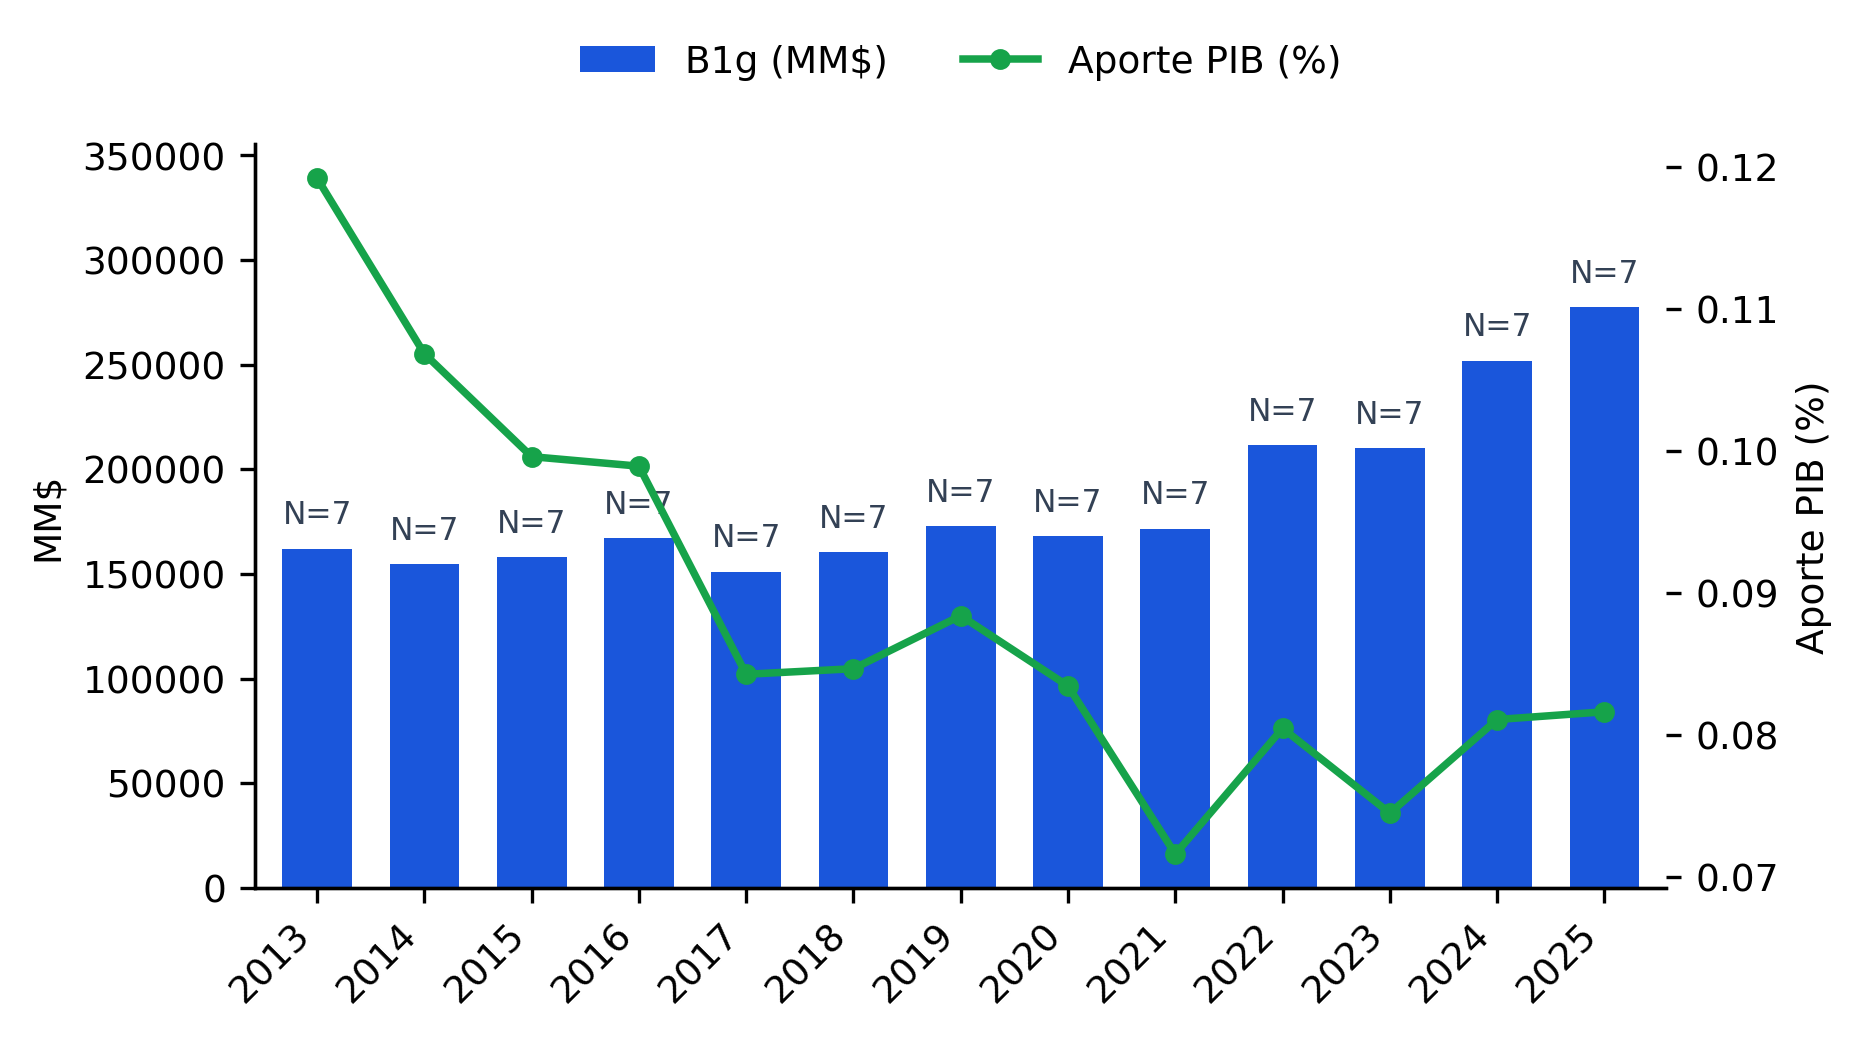
\includegraphics[width=\textwidth]{logos/figuras/CMF}
    \caption{VAB bruto (B1g) y aporte al PIB --- Segmento CMF.
    Las 7~CAC supervisadas muestran una tendencia creciente
    sostenida, con N\,=\,7 en todos los años del período
    2013--2025.}
    \label{fig:dash_cmf}
\end{figure}

La tendencia decreciente de la línea de aporte al PIB no
refleja una contracción del sector, sino el crecimiento
más acelerado de la economía chilena en el mismo período.
El VAB de las CAC CMF creció un 71\,\% en términos
nominales entre 2013 y 2025, pero el PIB nacional lo hizo
a un ritmo superior, reduciendo la participación relativa
del segmento de 0,119\,\% a 0,082\,\%.
\begin{figure}[H]
    \centering
    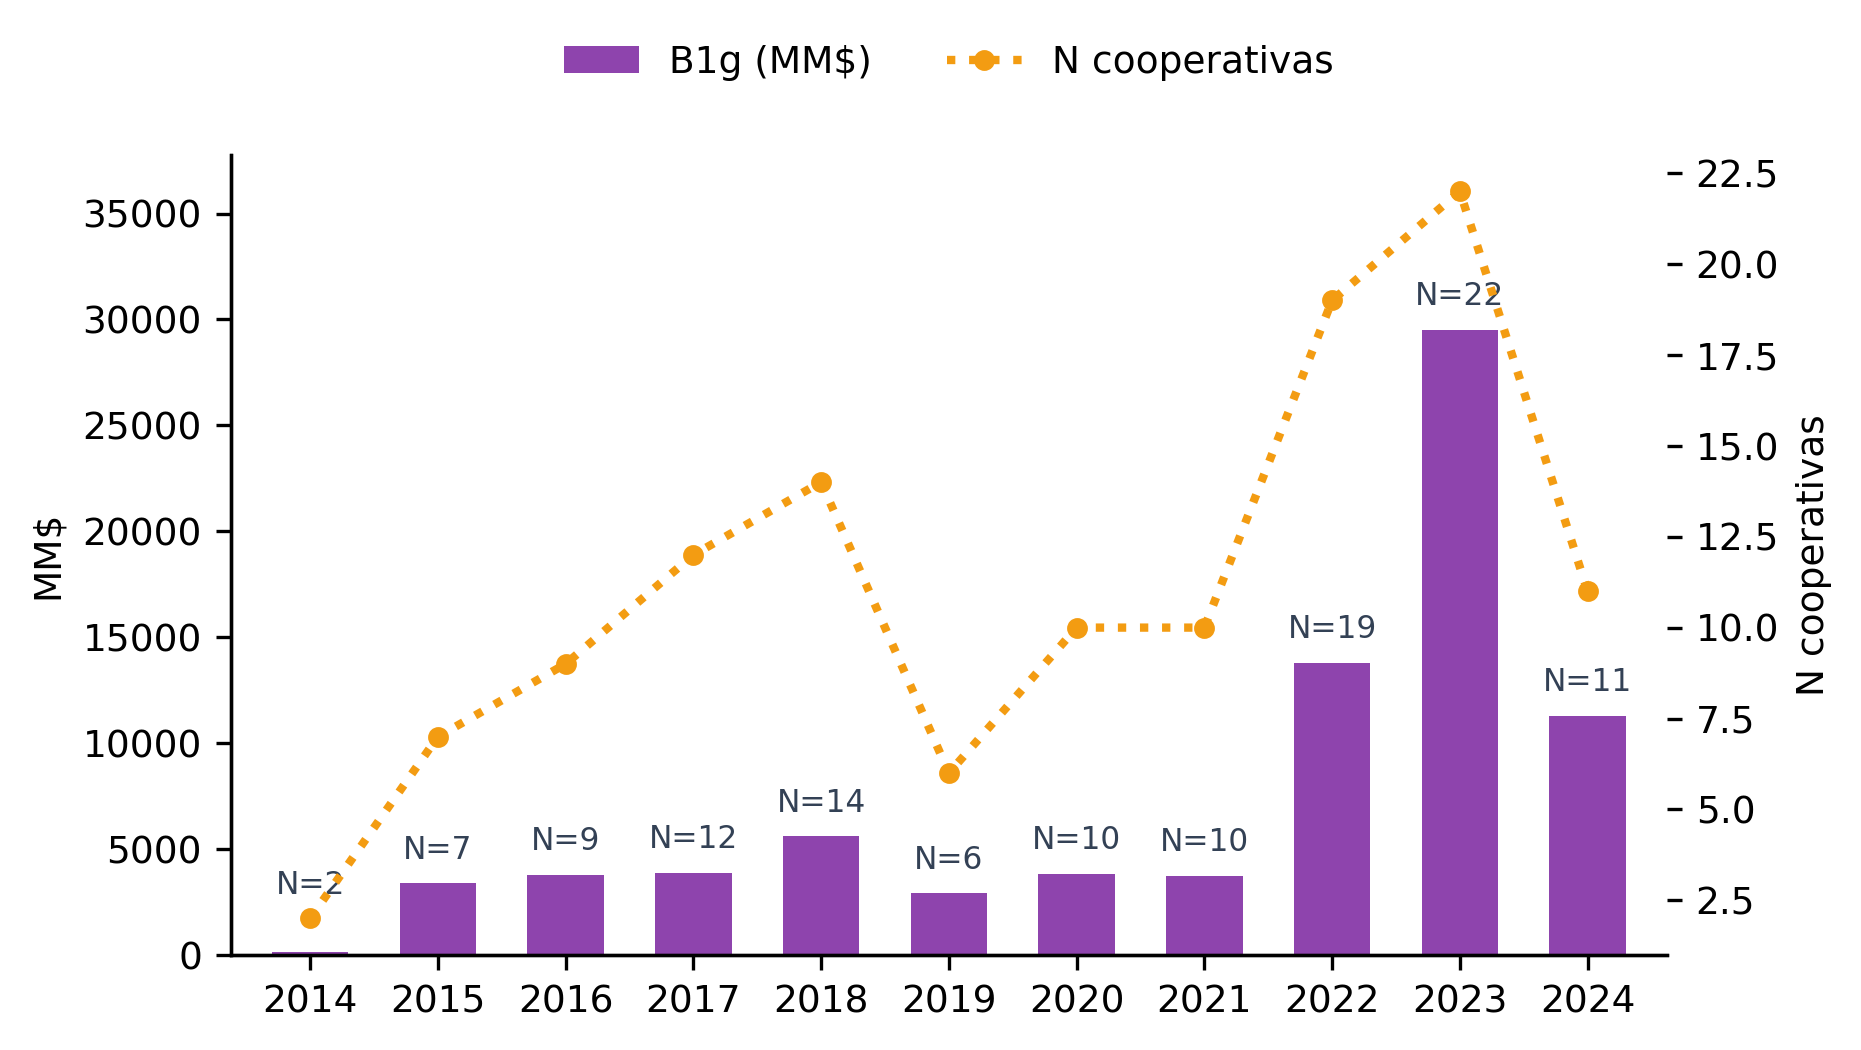
\includegraphics[width=\textwidth]{logos/figuras/DAES}
    \caption{VAB bruto (B1g) y número de cooperativas con dato
    --- Segmento DAES. El N variable por año refleja la
    disponibilidad de memorias en el portal DAES, período
    2014--2024.}
    \label{fig:dash_daes}
\end{figure}

La trayectoria del segmento DAES refleja dos fenómenos
simultáneos: el crecimiento real del VAB sectorial y el
aumento progresivo de la cobertura del panel. Entre 2014
y 2023 el número de CAC con dato disponible pasó de
2~a~22, lo que implica que parte del incremento observado
en B1g responde a la incorporación de nuevas entidades al
panel y no necesariamente a una expansión de la actividad
de las cooperativas ya presentes. La caída de 2024
(N\,=\,11) ilustra el efecto inverso: una reducción en la
disponibilidad de memorias ese año comprime el agregado
sectorial independientemente de lo que ocurra con la
actividad real. Por esta razón, las comparaciones
interanuales del segmento DAES deben interpretarse
controlando por N, y los niveles agregados constituyen
cotas inferiores del VAB real del segmento en cada año.
\begin{figure}[H]
    \centering
    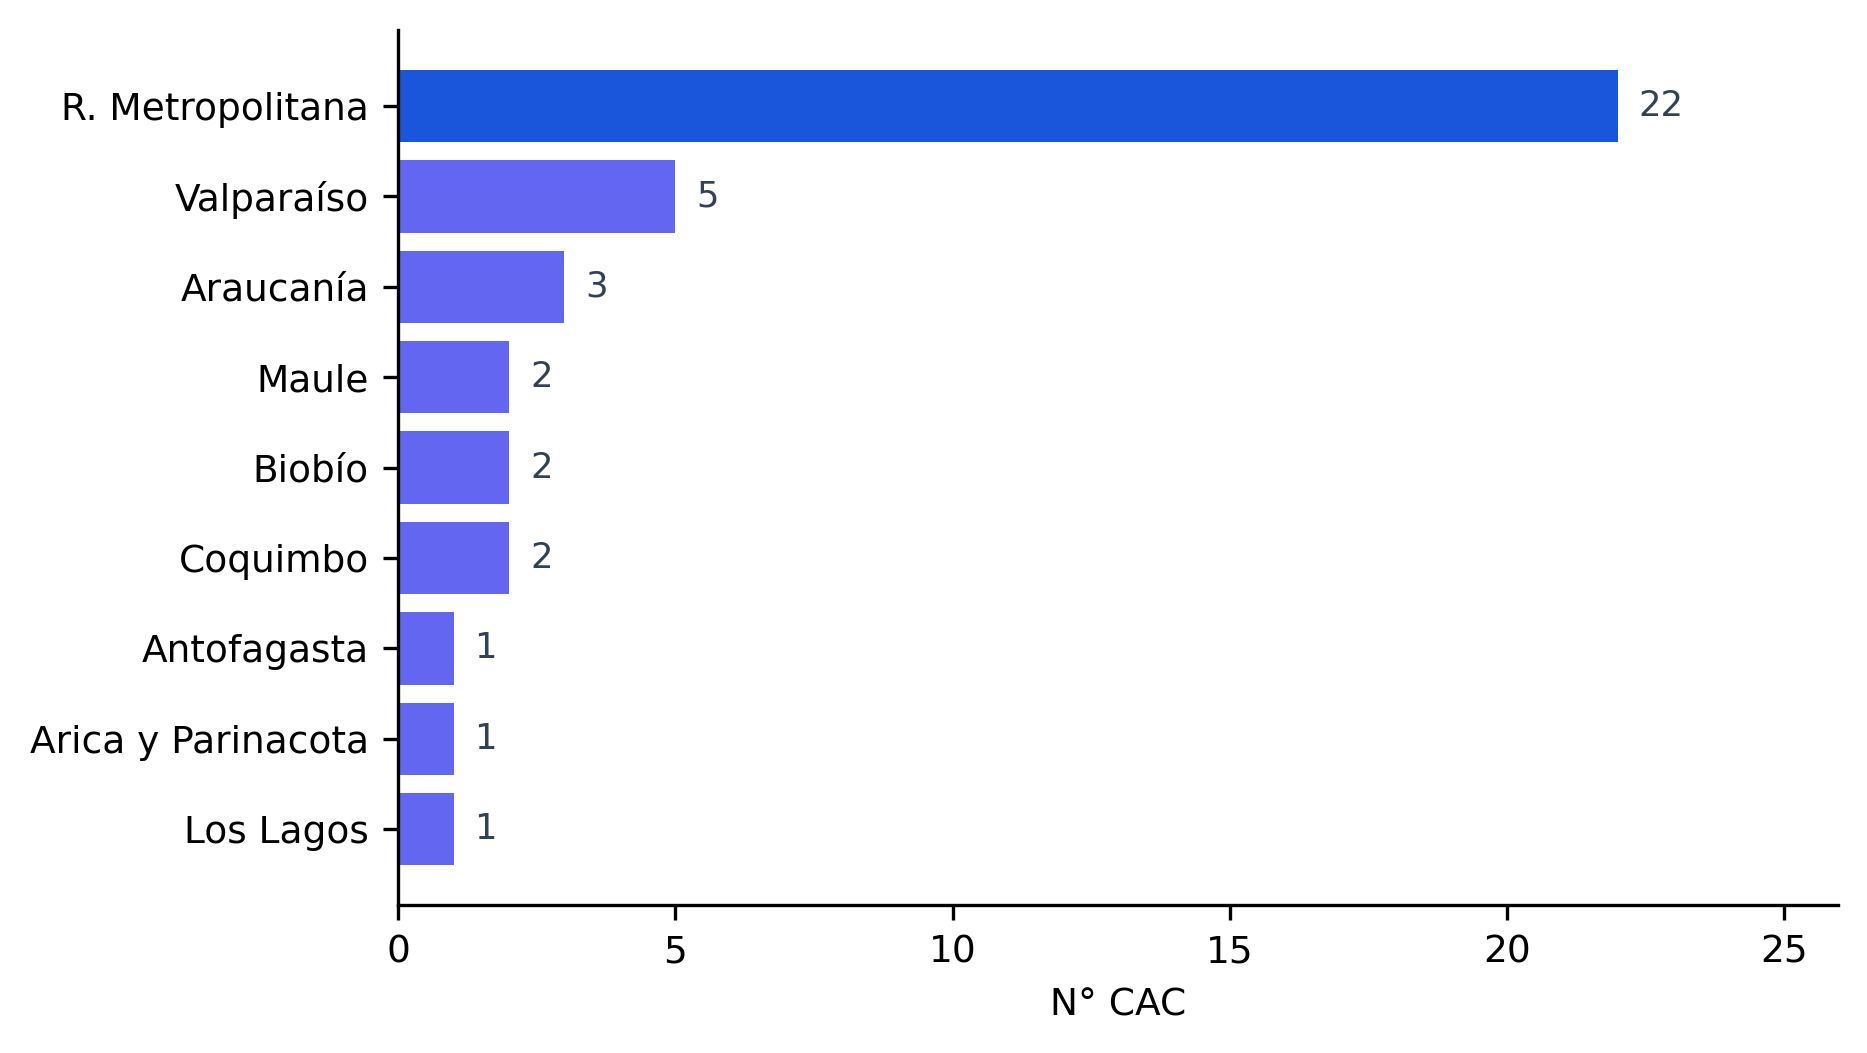
\includegraphics[width=0.7\textwidth]{logos/figuras/dash_regional2}
    \caption{Distribución regional de las CAC vigentes.
    La Región Metropolitana concentra 22 de las
    39~cooperativas del universo DAES + CMF.}
    \label{fig:dash_regional}
\end{figure}

La distribución geográfica del sector CAC muestra una
fuerte concentración en la Región Metropolitana, que
alberga 22 de las 39~cooperativas vigentes del universo
DAES + CMF, equivalente al 56\,\% del total. Valparaíso
y la Araucanía son las siguientes regiones con mayor
presencia, con 5 y 3~CAC respectivamente. El resto de
las regiones cuenta con una o dos cooperativas. Esta
concentración es consistente con el patrón general de
la actividad financiera cooperativa en Chile, donde las
zonas de mayor densidad poblacional y actividad
económica tienden a concentrar la mayor parte de las
instituciones del sector.
% ============================================================
\section{Limitaciones de los resultados}
\label{sec:limitaciones}
% ============================================================

Los resultados presentados están sujetos a cuatro
limitaciones principales, heredadas de las brechas de
información documentadas en la sección~\ref{subsec:supuestos-limitaciones}:

\begin{enumerate}

  \item \textbf{Cobertura parcial del universo DAES.}
  El panel nunca cubre la totalidad de las 35~CAC en un
  mismo año. Los agregados sectoriales son cotas inferiores
  del aporte real del segmento.

  \item \textbf{Supuesto de consumo intermedio uniforme.}
  El coeficiente $\alpha = 0{,}3776$ se aplica de forma
  homogénea a todas las CAC, independiente de su tamaño o
  estructura de costos. Cooperativas muy pequeñas pueden
  tener razones CI/P distintas al promedio sectorial.

  % DESPUÉS:
  \item \textbf{Incomparabilidad temporal entre segmentos.}
  El segmento DAES cubre 2014--2024 con cobertura anual variable y el 
  segmento CMF cubre 2013--2025 con cobertura completa. Por esta razón, la suma directa de ambos segmentos presentada en la sección~\ref{sec:agregado-total} no constituye una medición rigurosa y exacta del aporte total del sector, sino una aproximación de orden de magnitud que subestima el aporte real en los años en que el panel DAES no cubre la totalidad del universo de CAC. Esta cifra agregada se reporta con fines ilustrativos y de validación externa (sección~\ref{subsec:validacion-cmf}), y debe interpretarse con esa salvedad y no como una estimación exacta comparable año a año.



  \item \textbf{Ausencia de empleo para el segmento DAES.}
  La variable PEP (trabajadores) solo está disponible para
  12~CAC con presencia en la serie de tiempo del SII. Para
  las 26~CAC restantes del segmento DAES no existe dato de
  empleo en ninguna fuente administrativa, lo que impide
  calcular el indicador de productividad laboral (B1g/PEP)
  para el agregado sectorial.

\end{enumerate}